\textbf{COLUNI 2022 -- Questão 21}\par\medskip Leia o texto a seguir.

\par

% COLUNI-AUTO-FIGURES-BEGIN
\begin{figure}[htbp]
\centering
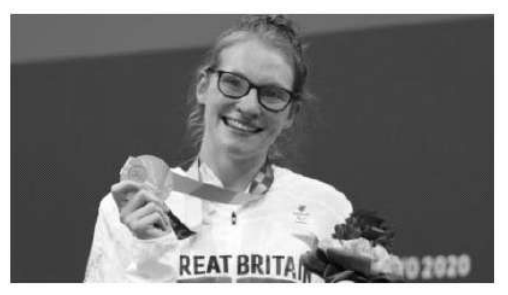
\includegraphics[width=0.95\linewidth]{static/simulados/coluni/figuras/2022/questao-21/figura-1.png}
\end{figure}
% COLUNI-AUTO-FIGURES-END

\begin{center}\textbf{Becky Redfern: The 'tough ride' to becoming a Paralympic silver medallist}\end{center}

\textbf{\underline{From the section}}  \textbf{\underline{Disability Sport}}

\textbf{Becky Redfern said it was "an incredible feeling" to win Paralympic silver in the SB13 100m breaststroke, just over a year after giving birth to her first child.}

The 21-year-old Briton thought her swimming career "was over" when she discovered she was pregnant. Redfern was able to compete in Tokyo because the Games were postponed for 12 months. "It has been a tough ride but I am just so happy right now," she said. "I am so proud of myself for everything that I have put myself through in the last couple of years and everything I've achieved today." The Rio 2016 silver medallist and 2019 world champion led at halfway on Wednesday but was overhauled by Germany's Elena Krawzow, who won by 0.64 seconds as Redfern clocked one minute 14.10secs. Redfern, who is visually impaired, gave birth to son Patrick in July 2020. "When I found out I was pregnant, I thought that my swimming career was done, it was over," she said. But for Redfern, the 12-month delay to the Paralympics because of Covid-19 "felt like fate, like they'd been postponed for me - I need to go and prove myself, they're waiting for me". Although swimming pools were forced to close, British Swimming hired a hot tub for her to train in at home during lockdown. However, preparing for Tokyo hasn't been her biggest challenge of the past year. "Being a mum is so hard, it's the hardest thing I've ever had to do," she told BBC Radio 5 Live. "To top it off with having to race and train - my son's just turned one and isn't sleeping through the night so I'm not getting the recovery time." Redfern said she could not wait to be reunited with Patrick so she could "give him a massive cuddle". She added: "He won't remember it, he's only one, but he will have all these memories to look back on and I know that he'll be proud of his mummy."

Disponível em: https://www.bbc.com/sport/disability-sport/58411534. Acesso em: 01 set. 2021. (Adaptado).

Com base no texto, analise as alternativas a seguir:

\par

I. Becky Redfern pensou que sua carreira havia acabado por causa da gravidez.\par
II. Se não fosse pela Covid-19, Becky Redfern não teria participado das paraolimpíadas de Tokyo.\par
III. Becky Redfern foi medalhista nas paraolimpíadas do Rio.\par
IV. O maior desafio na vida da medalhista foi se preparar para as paraolimpíadas.

\par

Está CORRETO o que se afirma em:

\begin{enumerate}
\item I, II, III e IV.
\item I e II, apenas.
\item I, II e III, apenas.
\item I, III e IV, apenas.\end{enumerate}
